\documentclass{beamer}
\usepackage[utf8]{inputenc}

\usetheme{Madrid}
\usecolortheme{default}
\usepackage{amsmath,amssymb,amsfonts,amsthm}
\usepackage{txfonts}
\usepackage{tkz-euclide}
\usepackage{listings}
\usepackage{adjustbox}
\usepackage{array}
\usepackage{tabularx}
\usepackage{gvv}
\usepackage{lmodern}
\usepackage{circuitikz}
\usepackage{tikz}
\usepackage{graphicx}
\usepackage[T1]{fontenc}
\usepackage[utf8]{inputenc}

\lstset{
  language=Python,
  basicstyle=\ttfamily\small,
  breaklines=true,
  literate={λ}{{$\lambda$}}1
}



\setbeamertemplate{page number in head/foot}[totalframenumber]

\usepackage{tcolorbox}
\tcbuselibrary{minted,breakable,xparse,skins}



\definecolor{bg}{gray}{0.95}
\DeclareTCBListing{mintedbox}{O{}m!O{}}{%
  breakable=true,
  listing engine=minted,
  listing only,
  minted language=#2,
  minted style=default,
  minted options={%
    linenos,
    gobble=0,
    breaklines=true,
    breakafter=,,
    fontsize=\small,
    numbersep=8pt,
    #1},
  boxsep=0pt,
  left skip=0pt,
  right skip=0pt,
  left=25pt,
  right=0pt,
  top=3pt,
  bottom=3pt,
  arc=5pt,
  leftrule=0pt,
  rightrule=0pt,
  bottomrule=2pt,
  toprule=2pt,
  colback=bg,
  colframe=orange!70,
  enhanced,
  overlay={%
    \begin{tcbclipinterior}
    \fill[orange!20!white] (frame.south west) rectangle ([xshift=20pt]frame.north west);
    \end{tcbclipinterior}},
  #3,
}
\lstset{
    language=C,
    basicstyle=\ttfamily\small,
    keywordstyle=\color{blue},
    stringstyle=\color{orange},
    commentstyle=\color{green!60!black},
    numbers=left,
    numberstyle=\tiny\color{gray},
    breaklines=true,
    showstringspaces=false,
}
\begin{document}

\title 
{2.7.27}
\date{September 14,2025}


\author 
{Bhoomika V - EE25BTECH11015}




\frame{\titlepage}
\begin{frame}{Question}
\[
\text{Find the area of the triangle } ABC \text{ whose vertices are }\\ \\
\vec{A}(2,5),\; \vec{B}(4,7),\; \vec{C}(6,2).
\]
\end{frame}

\begin{frame}{The vertices of a triangle}
\begin{table}[H]    
  \centering
  \begin{tabular}{|c|c|}
\hline
\textbf{Name} & \textbf{Value} \\ \hline
$\vec{A}$ & $\myvec{2 & 1 \\0 & 3}$ \\ \hline
\end{tabular}

  \caption{Vectors}
  \label{Answers}
\end{table}
\end{frame}

\begin{frame}{The sides of the triangle }
\begin{align}
(\vec{A}-\vec{B})
&= \begin{bmatrix} 2 \\ 5 \\ 0 \end{bmatrix}
  - \begin{bmatrix} 4 \\ 7 \\ 0 \end{bmatrix}
= \begin{bmatrix} -2 \\ -2 \\ 0 \end{bmatrix},
\label{eq:AB} \\[6pt]
(\vec{A}-\vec{C})
&= \begin{bmatrix} 2 \\ 5 \\ 0 \end{bmatrix}
  - \begin{bmatrix} 6 \\ 2 \\ 0 \end{bmatrix}
= \begin{bmatrix} -4 \\ 3 \\ 0 \end{bmatrix}.
\label{eq:AC}
\end{align}
\end{frame}

\begin{frame}{Cross product}
Using \eqref{eq:AB} and \eqref{eq:AC}  The magnitude of the cross product is
\begin{align}
\big\lVert (\vec{A}-\vec{B}) \times (\vec{A}-\vec{C}) \big\rVert
&= \sqrt{0^2 + 0^2 + (-14)^2} = 14.
\label{eq:norm}
\end{align}
\end{frame}

\begin{frame}{area of triangle}
Therefore the area of triangle \(ABC\) is
\begin{align}
\text{ar}(\triangle ABC)
&= \tfrac{1}{2}\,\big\lVert (\vec{A}-\vec{B}) \times (\vec{A}-\vec{C}) \big\rVert
= \tfrac{1}{2}\times 14 = 7.
\label{eq:area}
\end{align}
\end{frame}

\begin{frame}[fragile]
    \frametitle{C Code - A function to find if triangle is right angled }

    \begin{lstlisting}
#include <stdio.h>
#include <math.h>

// Function to compute area of triangle using cross product
float triangle_area(float Ax, float Ay, float Az,
                    float Bx, float By, float Bz,
                    float Cx, float Cy, float Cz) {
    // Vectors AB and AC
    float ABx = Bx - Ax;
    float ABy = By - Ay;
    float ABz = Bz - Az;

    float ACx = Cx - Ax;
    float ACy = Cy - Ay;
    float ACz = Cz - Az;
     \end{lstlisting}
\end{frame}

\begin{frame}[fragile]
    \frametitle{C Code - A function to find if triangle is right angled }

    \begin{lstlisting}
 // Cross product AB × AC
    float cross_x = ABy*ACz - ABz*ACy;
    float cross_y = ABz*ACx - ABx*ACz;
    float cross_z = ABx*ACy - ABy*ACx;

    // Area = 0.5 * |cross product|
    float area = 0.5 * sqrt(cross_x*cross_x + cross_y*cross_y + cross_z*cross_z);

    printf("Area of triangle ABC = %.2f\n", area);
    return area;
}

     \end{lstlisting}
\end{frame}

\begin{frame}[fragile]
    \frametitle{Python Code}
    \begin{lstlisting}
import numpy as np
import matplotlib.pyplot as plt
import ctypes
import os

# --- Load the C library ---
try:
    c_lib = ctypes.CDLL('./code.so')
except OSError:
    print("Error: 'code.so' not found. Compile using: gcc -shared -o code.so -fPIC triangle.c")
    exit()

# Define argument and return types
c_lib.triangle_area.argtypes = [ctypes.c_float, ctypes.c_float, ctypes.c_float,
                                ctypes.c_float, ctypes.c_float, ctypes.c_float,
                                ctypes.c_float, ctypes.c_float, ctypes.c_float]
c_lib.triangle_area.restype = ctypes.c_float
    \end{lstlisting}
\end{frame}

\begin{frame}[fragile]
    \frametitle{Python Code}
    \begin{lstlisting}
# --- Given points (2D extended to 3D with z=0) ---
A = np.array([2, 5, 0], dtype=np.float32)
B = np.array([4, 7, 0], dtype=np.float32)
C = np.array([6, 2, 0], dtype=np.float32)

# --- Call C function ---
area = c_lib.triangle_area(A[0], A[1], A[2],
                           B[0], B[1], B[2],
                           C[0], C[1], C[2])
print(f" Area of triangle = {area:.2f}")

# --- Plotting in 2D ---
fig, ax = plt.subplots(figsize=(6,6))
    \end{lstlisting}
\end{frame}

\begin{frame}[fragile]
    \frametitle{Python Code}
    \begin{lstlisting}
# Plot triangle edges
ax.plot([A[0], B[0]], [A[1], B[1]], color="black")
ax.plot([B[0], C[0]], [B[1], C[1]], color="black")
ax.plot([C[0], A[0]], [C[1], A[1]], color="black")

# Fill triangle
ax.fill([A[0], B[0], C[0]], [A[1], B[1], C[1]], color="cyan", alpha=0.3)

# Points
ax.scatter(A[0], A[1], color="red", s=60)
ax.scatter(B[0], B[1], color="blue", s=60)
ax.scatter(C[0], C[1], color="green", s=60)

# Labels
ax.text(A[0]+0.1, A[1], "A(2,5)", color="red")
ax.text(B[0]+0.1, B[1], "B(4,7)", color="blue")
ax.text(C[0]+0.1, C[1], "C(6,2)", color="green")

    \end{lstlisting}
\end{frame}

\begin{frame}[fragile]
    \frametitle{Python Code}
    \begin{lstlisting}
# Area annotation
ax.text(3.5, 4.5, f"Area = {area:.2f}", color="purple", fontsize=12)

# Formatting
ax.set_xlabel("X-axis")
ax.set_ylabel("Y-axis")
ax.set_title("Triangle ABC in 2D plane")
ax.grid(True)
ax.set_aspect("equal")

plt.show()
        \end{lstlisting}
\end{frame}

\begin{frame}{Plot}
    \centering
    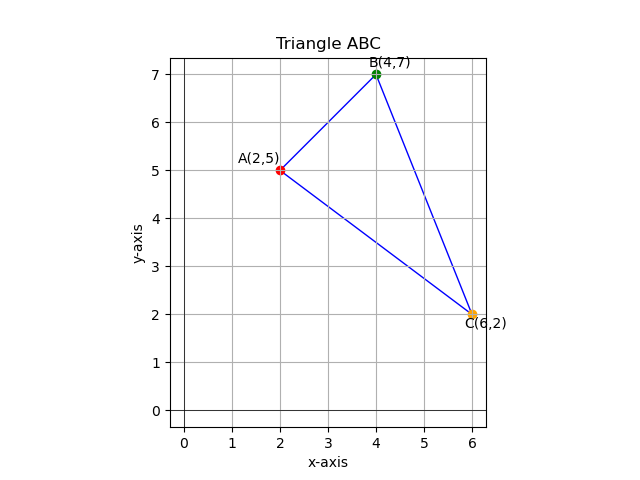
\includegraphics[width=\columnwidth, height=0.8\textheight, keepaspectratio]{Figs/Fig1.png}     
\end{frame}

\end{document}